\newpage

\subsection{Aufbau des Operationsbefehls}

\begin{minipage}[t]{1\textwidth}
	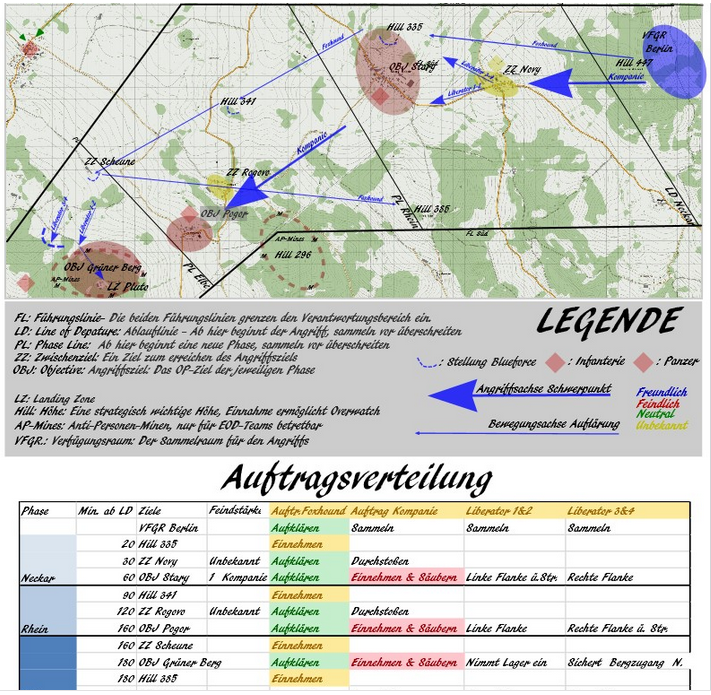
\includegraphics[width=\textwidth]{./Grafiken/KarteUndMarkierungen/OP-Befehl.png}
\end{minipage}

\begin{longtable}{|p{3cm}|p{1,8 cm}|p{2,7cm}|p{4cm}|p{1,5cm}|} 																											\hline
	Linien				&		Abkürzung			&		Bezeichnung				&			Anmerkung 									&		Beispiel 			\\ \hline
	Führungslinie			&		FL				&		Angrenzende Himmelsrichtung	&			Die Führungslinien grenzen \newline den Verantwortungsbereich und \newline das Operationsgebiet ein. & FL Nord, FL SW \\ \hline
	Line of Depature (Ablauflinie)&		LD				&		Großer Fluss				&			Beim Überschreiten beginnt der Angriff und die Kampfhandlung 	&	LD Rhein, LD Donau			\\ \hline
	Phase Line (Kordinierungs-Führungslinie) & PL				&		Kleinere Flüsse			&			Eine OP unterteilt sich in zwei- drei räumlich und zeitlich getrennte Phasen, markiert durch die Phasenlinien	& PL Neckar, PL Inn, PL Isar	\\ \hline
	Sicherungslinie 		&		SL 				&		Insel					&			Sicherungslinien, auf denen der Feind abzuwehren ist.		&	SL Rügen, SL Sylt			\\ \hline
\end{longtable}

\begin{longtable}{|p{3cm}|p{1,8 cm}|p{2,7cm}|p{4cm}|p{1,5cm}|} 																											\hline
	Räume			&		Abkürzung			&		Bezeichnung				&			Anmerkung 									&		Beispiel 			\\ \hline
	Casualty Collection Point (Verwundeten Sammelstelle) & CCP	& 		Verwundeten- sammelstelle mit VS und Geländebeschreibung versehen & Hier werden die Verwundeten gesammelt		& 		CCP Ruine, CCP Abdera	\\ \hline
	Verfügungsräume		&		VGR				&		Bundesländer, Bundesstaaten	&			Sammelraum pro Phase, der als Sicher gilt. Häufig gibt es nur einen VGR vor der LD. 	&	VGR Bayern, VGR Pfalz \\ \hline
	Brückenkopf			&		BR				&		Helden				&			Wassernahe Stellung/Anlandungszone  im feindlichen Gebiet (Brücke, Strand, Flussseite)	& BR Herakles, BR Odin, BR Thor \\ \hline
\end{longtable}

\begin{longtable}{|p{3cm}|p{1,8 cm}|p{2,7cm}|p{4cm}|p{1,5cm}|} 																											\hline
	Ziele und Topographie	&		Abkürzung			&		Bezeichnung				&			Anmerkung 									&		Beispiel 			\\ \hline
	Zwischenziel			&		ZZ				&		Eingekürzter Name des Ortes oder konkrete Beschreibung des Ziels	&	Zwischenziele sind optionale Ziele, je nach Schlachtverlauf zu erreichen. ZZ mit Nummer versehen!	& ZZ Lager \#1, ZZ Novograd \#1 \\ \hline
	Objective			&		OBJ				&		Eingekürzter Name des Ortes oder konkrete Beschreibung des Ziels	&	Die Hauptziele der Operation		&		OBJ Abdera, OBJ Airport	\\ \hline
	Hill (Hügel/Anhöhe)		&		Hill				&		Hügel immer mit aktueller Höhenangabe versehen.	&	Stratgisch wichtige Anhöhen					&		Hill 136			\\ \hline
	Geländemarke		&		GM				&		Beschreibung, Ein, maximal zwei Wörter (Adjektiv, Subjekt)	&	Besondere Geländeeigenschaften werden beschrieben.	& 	GM Kugelbaum, GM tiefe Senke \\ \hline
\end{longtable}